\documentclass{webofc}
\usepackage[varg]{txfonts}
\usepackage{amsmath}

% Common
\newcommand{\kjpsi}{\ensuremath{(\textrm{J}/\Psi{\rightarrow})}\xspace}
\newcommand{\ellell}{\ensuremath{\ell^+\ell^-}\xspace}
\newcommand{\ee}{\ensuremath{\textrm{e}^+\textrm{e}^-}\xspace}
\newcommand{\mumu}{\ensuremath{\mu^+\mu^-}\xspace}
\newcommand{\bto}{\ensuremath{\textrm{b}{\rightarrow}}\xspace}
\newcommand{\btok}{\ensuremath{\textrm{B}^+{\rightarrow}\textrm{K}^+}\xspace}
\newcommand{\btokst}{\ensuremath{\textrm{B}^0{\rightarrow}\textrm{K}^*}\xspace}
\newcommand{\btokstar}{\ensuremath{\textrm{B}^{+(0)}{\rightarrow}\textrm{K}^{(*)}}\xspace}
% B->Kll
\newcommand{\btokll}{\ensuremath{\btok\ellell}\xspace}
\newcommand{\btokmm}{\ensuremath{\btok\mumu}\xspace}
\newcommand{\btokee}{\ensuremath{\btok\ee}\xspace}
\newcommand{\btokjpsill}{\ensuremath{\btok\kjpsi\ellell}\xspace}
\newcommand{\btokjpsimm}{\ensuremath{\btok\kjpsi\mumu}\xspace}
\newcommand{\btokjpsiee}{\ensuremath{\btok\kjpsi\ee}\xspace}
\newcommand{\rk}{\ensuremath{R_{\textrm{K}}}\xspace}
% B->K*ll
\newcommand{\btokstll}{\ensuremath{\btokst\ellell}\xspace}
\newcommand{\btokstmm}{\ensuremath{\btokst\mumu}\xspace}
\newcommand{\btokstee}{\ensuremath{\btokst\ee}\xspace}
\newcommand{\btokstjpsill}{\ensuremath{\btokst\kjpsi\ellell}\xspace}
\newcommand{\rkst}{\ensuremath{R_{\textrm{K}^*}}\xspace}
% B->K(*)ll
\newcommand{\btokstarll}{\ensuremath{\btokstar\ellell}\xspace}
\newcommand{\btokstarmm}{\ensuremath{\btokstar\mumu}\xspace}
\newcommand{\btokstaree}{\ensuremath{\btokstar\ee}\xspace}
\newcommand{\btokstarjpsill}{\ensuremath{\btokstar\kjpsi\ellell}\xspace}
% b->sll, etc
\newcommand{\bsll}{\ensuremath{\bto\textrm{s}\ell\ell}\xspace}
\newcommand{\bclnu}{\ensuremath{\bto\textrm{c}\ell\nu}\xspace}
\newcommand{\btomux}{\ensuremath{\bto\mu\textrm{X}}\xspace}
\newcommand{\bctomux}{\ensuremath{{\bto}\textrm{c}{\rightarrow}\mu\textrm{X}}\xspace}
\newcommand{\btoctomux}{\ensuremath{{\bto}(\textrm{c}{\rightarrow})\mu\textrm{X}}\xspace}
\newcommand{\bstomm}{\ensuremath{\textrm{B}^0_{(s)}{\rightarrow}\mumu}\xspace}
% Misc
\newcommand{\bbar}{\ensuremath{\textrm{b}\bar{\textrm{b}}}\xspace}
\newcommand{\pt}{\ensuremath{p_\textrm{T}}\xspace}
\newcommand{\ate}{\ensuremath{\mathcal{A}\epsilon}\xspace}
\newcommand{\instlumi}{\ensuremath{\mathcal{L}_{\textrm{inst}}}\xspace}
\newcommand{\cms}{\ensuremath{\,\textrm{cm}^{-2}\textrm{s}^{-1}}\xspace}
\newcommand{\ipsig}{\ensuremath{\textrm{IP}_{\textrm{sig}}}\xspace}
\newcommand{\gbs}{\ensuremath{\,\textrm{GB}\,\textrm{s}^{-1}}\xspace}

\begin{document}

\title{Recording and reconstructing 10 billion unbiased b hadron
  decays in CMS}

\author{ 
  \firstname{Robert} \lastname{Bainbridge}\inst{1}, 
  \lastname{on behalf of the CMS Collaboration}\thanks{
    \email{cms-phys-conveners-BPH@cern.ch}
  } 
}
\institute{Imperial College London, SW7 2AZ, UK}

\abstract{%
  The CMS experiment has recorded a high-purity sample of 10 billion
  unbiased b hadron decays. The CMS trigger and data acquisition
  systems were configured to deliver a custom data stream at an
  average throughput of 2\gbs, which was "parked" prior to
  reconstruction. The data stream was defined by Level-1 and high
  level trigger algorithms that operated at peak trigger rates in
  excess of 50 and 5~kHz, respectively. New algorithms have been
  developed to reconstruct and identify electrons with high efficiency
  at transverse momenta as low as 0.5 GeV. The trigger strategy and
  electron reconstruction performance were validated with pilot
  processing campaigns. The accumulation and reconstruction of this
  data set, now complete, were delivered without significant impact on
  the core physics programme of CMS. This unprecedented sample
  provides a unique opportunity for physics analyses in the flavour
  sector and beyond.
} 

\maketitle

\section{Introduction}
\label{sec:1}

In recent years, a number of experimental results related to lepton
universality tests in b hadron decays have yielded
measurements~\cite{} that are in tension with expected values from the
standard model. The cited measurements, performed by the
BaBar~\cite{babar}, Belle~\cite{belle}, and LHCb~\cite{lhcb}
Collaborations, are for both \bsll and \bclnu transitions and the
individual measurements exhibit deviations in the range 2--4$\sigma$.
Collectively, they may be the first indications of the violation of
lepton flavour universality (LFU)~\cite{hflav-rdrdst,
  altmannshofer}. The confirmation of LFU violation would be a
striking proof of the existence of physics beyond the SM. A key
experimental observable \rk is defined by the double ratio %
\begin{equation}
  \rk =
  \frac{\mathcal{B}[\btokmm]\,/\,\mathcal{B}[\btokjpsimm]}{\mathcal{B}[\btokee]\,/\,\mathcal{B}[\btokjpsiee]}, 
  \label{equ:1}
\end{equation}
where the numerator and denominator are ratios of the branching
fractions for the resonant \btokjpsill and nonresonant \btokll decays
in the muonic (electronic) channel, respectively.\footnote{The
  \btokstarll and \btokstarjpsill notation implies charge
  conjugation.} The \rkst observable is similarly defined using the
branching fractions for the resonant \btokstll and nonresonant
\btokstjpsill decays. The \rk and \rkst observables are known with
high theoretical precision~\cite{} as a function of the 4-momentum
transfer of the dilepton system, $q^2(\ell\ell)$, and thus are ideal
probes for the presence of new-physics processes in rare decays due to
\bsll transitions.

Results related to lepton universality from the CMS
experiment~\cite{cms-expt} are thus far limited: examples include the
measurements of branching fractions for \bstomm~\cite{bsmumu} and
angular analyses of \btokstmm decays ~\cite{p5prime-cms}. The CMS
trigger system~\cite{cms-trigger} comprises a two-tier system that
enables algorithms on a level-1 (L1) subsystem of custom hardware
processors and a software-based high-level trigger (HLT) subsystem
that runs on a farm of processors. The system already implements the
required algorithms to efficiently record samples of b hadron decays
in muonic final states with high purity. However, there is no
corresponding trigger logic that can be used to collect an adequate
sample of \btokstaree decays. This limitation has thus far prevented
the measurements of \rk and \rkst by the CMS Collaboration.

A novel trigger and "B parking" strategy was deployed during the data
taking period in 2018, which has enabled the accumulation and
reconstruction of 10~B unbiased b hadron decays from which the
measurements of \rk and \rkst may be derived. The data streams that
serve the core physics programme of CMS are promptly reconstructed at
the CERN Tier0 data centre, and are generally available within 48
hours for physics analysis. The new data stream has a trigger rate of
several kHz, which is beyond the standard processing capabilities of
the Tier0 centre. However, the trigger and data acquisition (DAQ)
systems have the ability to record nonstandard parked data streams to
extend the CMS physics programme~\cite{parking-dps}. These data
streams, typically defined by relaxed inclusive trigger requirements,
are not processed immediately by the CMS reconstruction software.
Instead, the data are temporarily stored in local buffers at Point~5
before being transferred---unprocessed---to permanent tape storage.
These data streams are processed at a later point in time, e.g.~during
an end-of-year or long shutdown of the LHC. The parked data streams
serve analyses with complementary or extended coverage
(e.g.~Ref.~\cite{alphat}) with respect to the core CMS physics
programme.

This sample of unbiased b hadron decays, unprecedented in its size,
provides a unique opportunity for the discovery of new-physics
processes, in the flavour sector and beyond, and it is complementary
to the high-\pt new-physics search programme of CMS. The trigger and B
parking strategy, a new electron reconstruction algorithm, and some
preliminary validation studies are described in the following
sections.

\section{Trigger strategy}
\label{sec:2}

The selection of \bbar events using a "tag-side" trigger logic in
order to accumulate a sample of unbiased "signal-side" b hadron decays
has been an important technique for analyses at B factories, LEP, and
hadron colliders. The natural decay channels for the signal-side b
hadron are unbiased by the trigger logic requirements imposed on the
tag-side decay. The logic is based on the presence of a single muon,
as semileptonic decays to muonic final states, \btoctomux, account for
${\approx}$20\% of all b hadron decays.

In CMS, the same tag-side technique, coupled with existing trigger
logic for muons, is used to record both the (signal-side) muonic and
electronic final states required by the \rk and \rkst measurements.
The CMS trigger logic has been tuned to record \btoctomux events with
a purity of ${\approx}80\%$, as described below. The \btokstarll
decays have branching fractions of $\mathcal{O}(10^{-7})$. Assuming an
acceptance times efficiency (\ate) of ${\approx}10\%$, a large sample
of $\mathcal{O}(10^{10})$ \bbar events is therefore required to obtain
$\mathcal{O}(100)$ events containing \btokstarmm or \btokstaree
decays. The expected yield, $N(\btokstarll)$, after the application of
a muon-based L1 trigger algorithm during data taking in 2018 can be
estimated by %
\begin{equation}
  N(\btokstarll) = f_{\textrm{B}} \times
  \mathcal{B}[\btokstarll] \times R_{\textrm{L1}} \times
  P_{\textrm{L1}} \times t_{\textrm{LHC}},
  \label{equ:2}  
\end{equation}
where $f_{\textrm{B}}$ is the fractional production rate of a
particular type of b hadron relative to all b hadrons (e.g.~0.4 for
$\textrm{B}^0$ and $\textrm{B}^\pm$); $R_{\textrm{L1}}$ is the rate
[kHz] of positive decisions by the L1 trigger logic; $P_{\textrm{L1}}$
is the purity of the event sample recorded by the L1 trigger logic,
assumed here to be 0.3; and $t_{\textrm{LHC}}$ is the duration of the
data taking period in 2018, assumed to be $7.8 \times 10^6~\textrm{s}$
(i.e.~six months of LHC operation with a duty cycle of 50\%). The
branching fraction for \btokll (\btokstll) is $4.5~(6.7) \times
10^{-7}$~\cite{}. Hence, assuming a L1 trigger rate of 10~kHz, the
total number of events with a positive L1 decision that contain a
signal-side \btokll (\btokstll) decay is estimated to be
${\approx}4000$ (${\approx}6000$).

The purity of the data stream is substantially improved through the
use of tailored muon algorithms in the HLT. Studies have identified
the two variables with the highest discriminating power to improve
purity while maintaining acceptance to the signal processes: the muon
\pt and the muon impact parameter (defined as the spatial distance
between the primary pp collision and the muon at its point of closest
approach), expressed in terms of its measurement significance, \ipsig.
The latter variable leverages the lifetime of the
$\textrm{B}^{\pm(0)}$ meson and the characteristic displacement of the
muon. The improved purity provided by the HLT algorithm is an
important factor in controlling the total rate at which events are
recorded by the CMS trigger system and written to tape.

The trigger strategy aims to maximise the number of \btokstarll events
recorded during 2018 while ensuring that the ability of the CMS
trigger and DAQ systems to deliver the core physics programme is
unaffected. This is achieved by taking advantage of an increase in
idle online computing resources as the instantaneous luminosity
\instlumi decreases during each LHC fill. Specifically, as \instlumi
decreases, the L1 and HLT trigger rates decrease, and the per-event
processing load also decreases as a consequence of a reduced number of
additional pp interactions within the same bunch crossing as the
primary interaction (pileup).

\begin{table}[!b]
  \small%\scriptsize
  \centering 
  % L760 of webofc.cls is now commented, to left-justify table captions
  \caption{Summary of the tag-side muon trigger requirements
    imposed by the L1 and HLT algorithms: the L1 and HLT muon \pt
    thresholds, and the HLT muon impact parameter significance
    \ipsig. Also shown are the trigger purity and peak trigger
    rate. All values are shown as a function of the peak \instlumi.
    Table contents taken from Ref.~\cite{bpark-dps}.} 
  \label{tab:1}
  \begin{tabular}{ccccccc}
    \hline
    Settings & Peak \instlumi  & L1 $\mu$ \pt  & HLT $\mu$ \pt & HLT $\mu$ \ipsig & Purity & Peak Rate \\
             & $[10^{34}\cms]$ & thresh. [GeV] & thresh. [GeV] & threshold        &        & [kHz]     \\
    \hline
    1        & 1.7             & 12            & 12            & 6                & 0.92   & 1.5       \\
    2        & 1.5             & 10            & 9             & 6                & 0.87   & 2.8       \\
    3        & 1.3             & 9             & 9             & 5                & 0.86   & 3.0       \\
    4        & 1.1             & 8             & 8             & 5                & 0.83   & 3.7       \\
    5        & 0.9             & 7             & 7             & 4                & 0.59   & 5.4       \\
    \hline
  \end{tabular}
\end{table}

Table~\ref{tab:1} summarises the tag-side muon trigger requirements
imposed by the L1 and HLT algorithms. The L1 logic requires the
presence of a muon that satifies $|\eta| < 1.5$, which helps to
control rate and also improves the acceptance for the signal-side
\btokstarll decays. Both the L1 and HLT requirements are relaxed
through a series of settings that progressively increase the rate at
which the CMS trigger system results in a positive decision with only
a moderate reduction in purity. The purity, estimated from simulation,
is found to be in the range 0.59--0.92, with an average value of
${\approx}0.75$ that has been validated against data by reconstructing
$\textrm{D}^{*+}$ candidates from the decay $\textrm{B}^0
{\rightarrow} \textrm{D}^{*+}\mu\nu {\rightarrow}
(\textrm{D}^{0}\pi_{\textrm{soft}})\mu\nu {\rightarrow}
(\textrm{K}^+\pi\pi_{\textrm{soft}})\mu\nu$. The trigger rates of the
L1 and HLT system peak at values of ${\approx}50$~kHz and 5.4~kHz,
respectively. The highest rates are observed late in an LHC fill,
which results in a pileup value of ${\approx}20$ when averaged over an
entire LHC fill. This value is a factor ${\approx}2$ lower than that
typically observed for the standard physics data streams of CMS.

Figure~\ref{fig:1} shows the trigger rate of the CMS L1 system as a
function of time during an LHC fill in 2017 (left) and 2018 (right).
The left panel illustrates how the total rate decreases with time, as
a consequence of the decreasing \instlumi during the LHC fill. The
right panel illustrates how the total rate is maintained close to the
optimum value of ${\approx}$90~kHz by evolving the settings, as
defined in Table~\ref{tab:1}. The left panel of Fig.~\ref{fig:2} shows
the trigger rates of the CMS HLT system as a function of time during
an LHC fill in 2018, for both the standard physics and B parking
streams. Sharp increases in the rate for the B parking stream occur
throughout the LHC fill, as the settings are evolved, while the rate
decreases monotonically for the standard physics data streams.

\begin{figure}[!t]
  \centering
  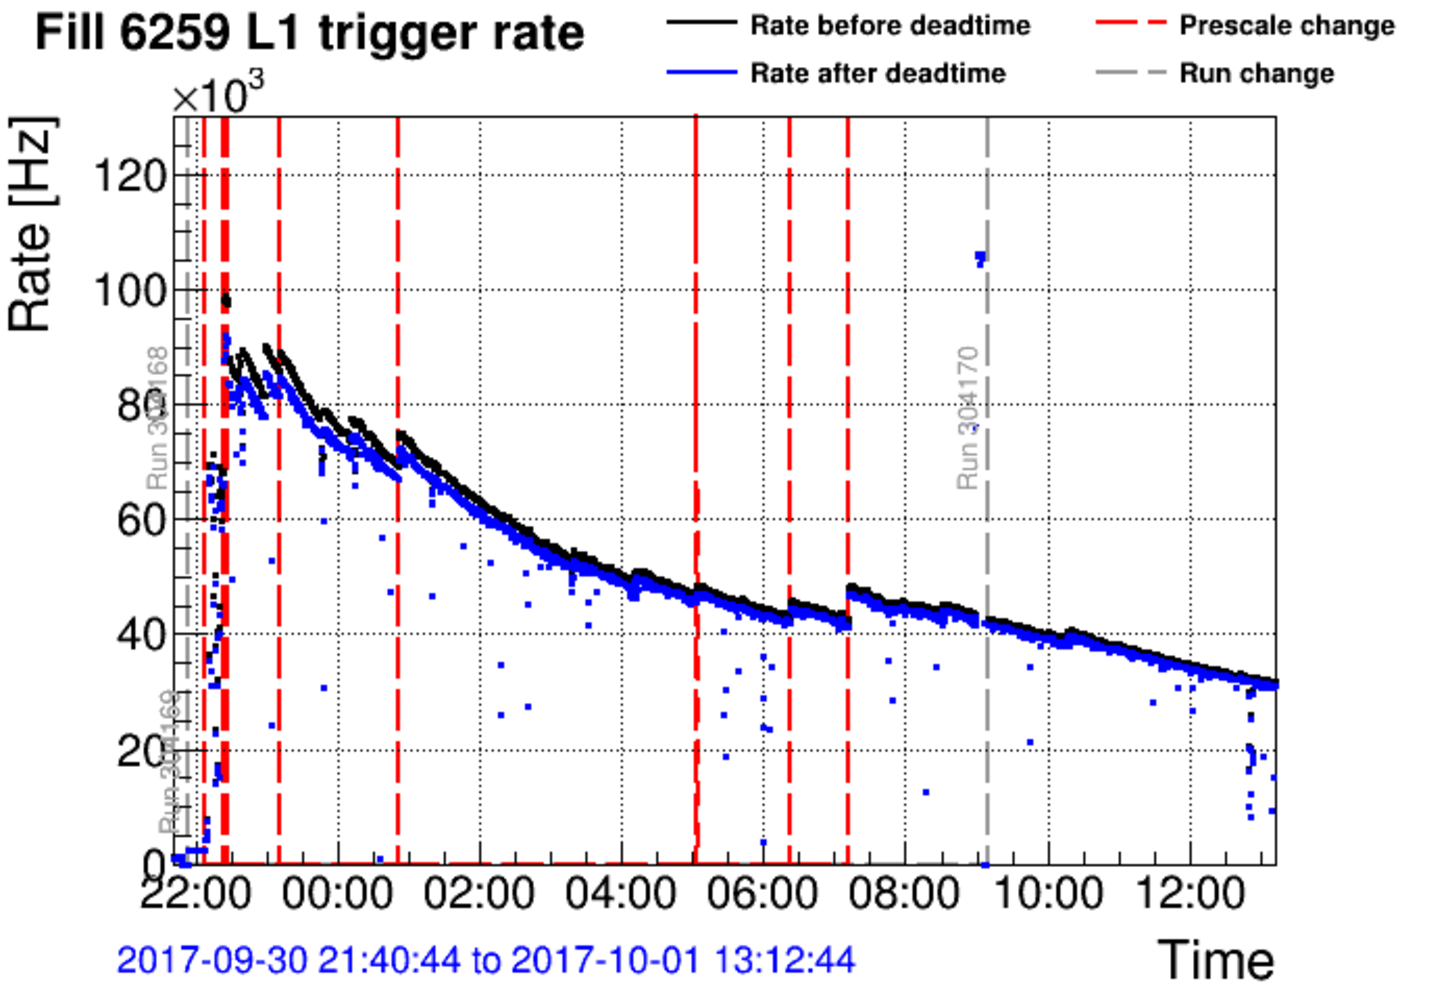
\includegraphics[width=0.45\textwidth]{CMS-DP-2019-XXX_S02}
  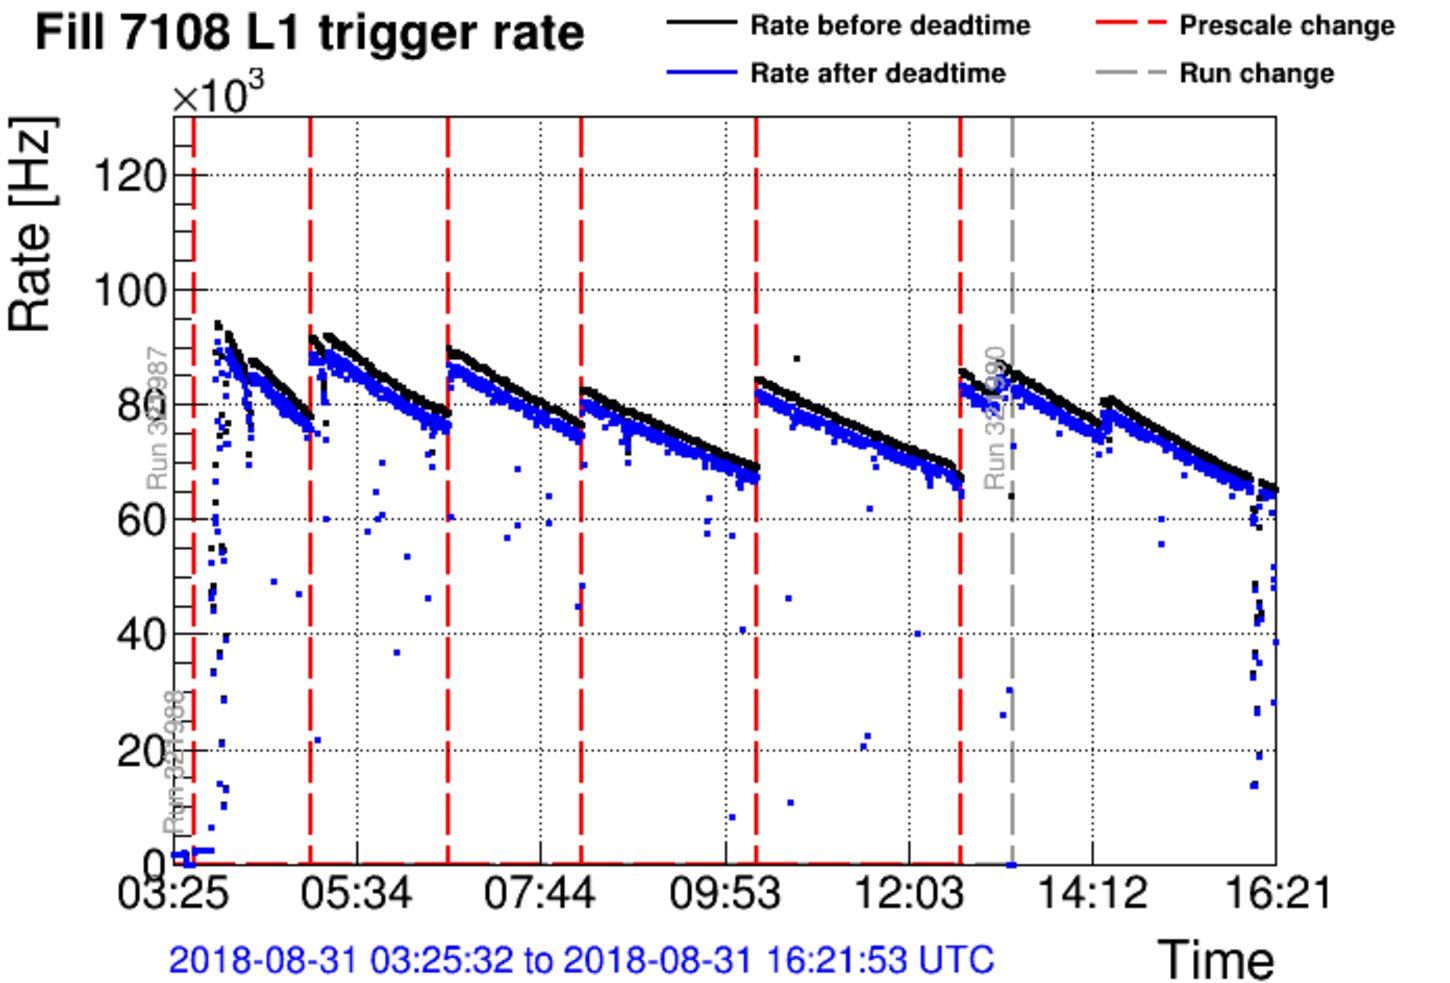
\includegraphics[width=0.45\textwidth]{CMS-DP-2019-XXX_S03}
  \caption{Rate of the CMS L1 trigger (blue data points), as a
    function of time, during an LHC fill in (\textbf{left panel}) 2017
    and (\textbf{right panel}) 2018. The time intervals cover 13--15
    hours. Changes in the run number and settings (prescale column)
    are indicated by vertical grey and red dashed lines,
    respectively. Taken from Ref.~\cite{bpark-dps}.}  
  \label{fig:1}
\end{figure}

\begin{figure}[!t]
  \centering
  % \sidecaption
  % L783 of webofc.cls is now commented, to remove ragged-right sidecaption option
  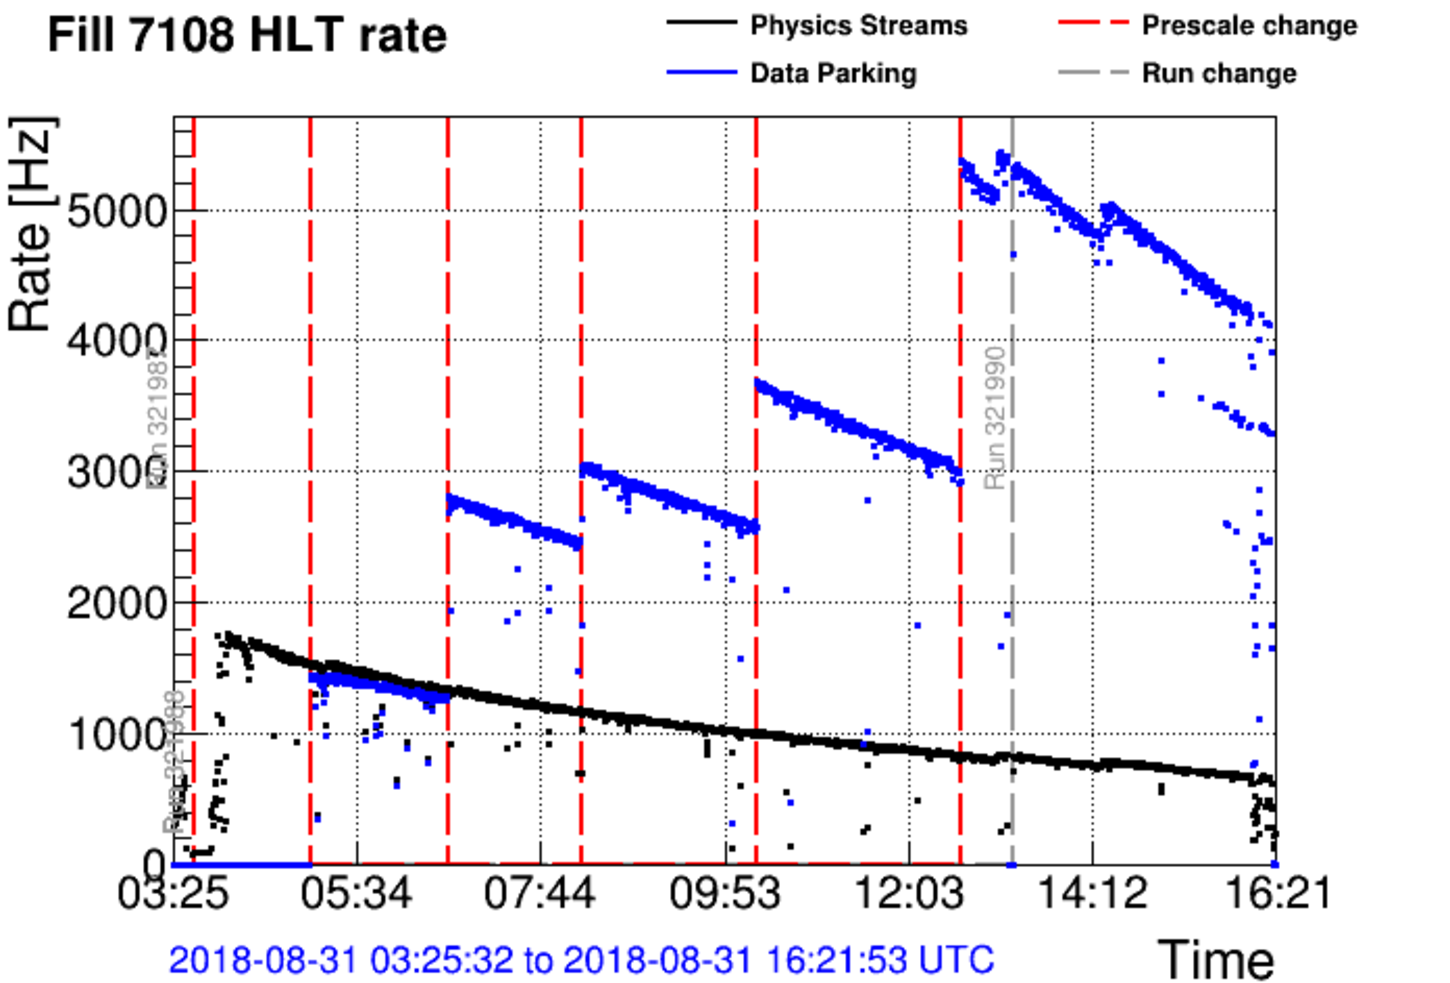
\includegraphics[width=0.45\textwidth]{CMS-DP-2019-XXX_S04}
  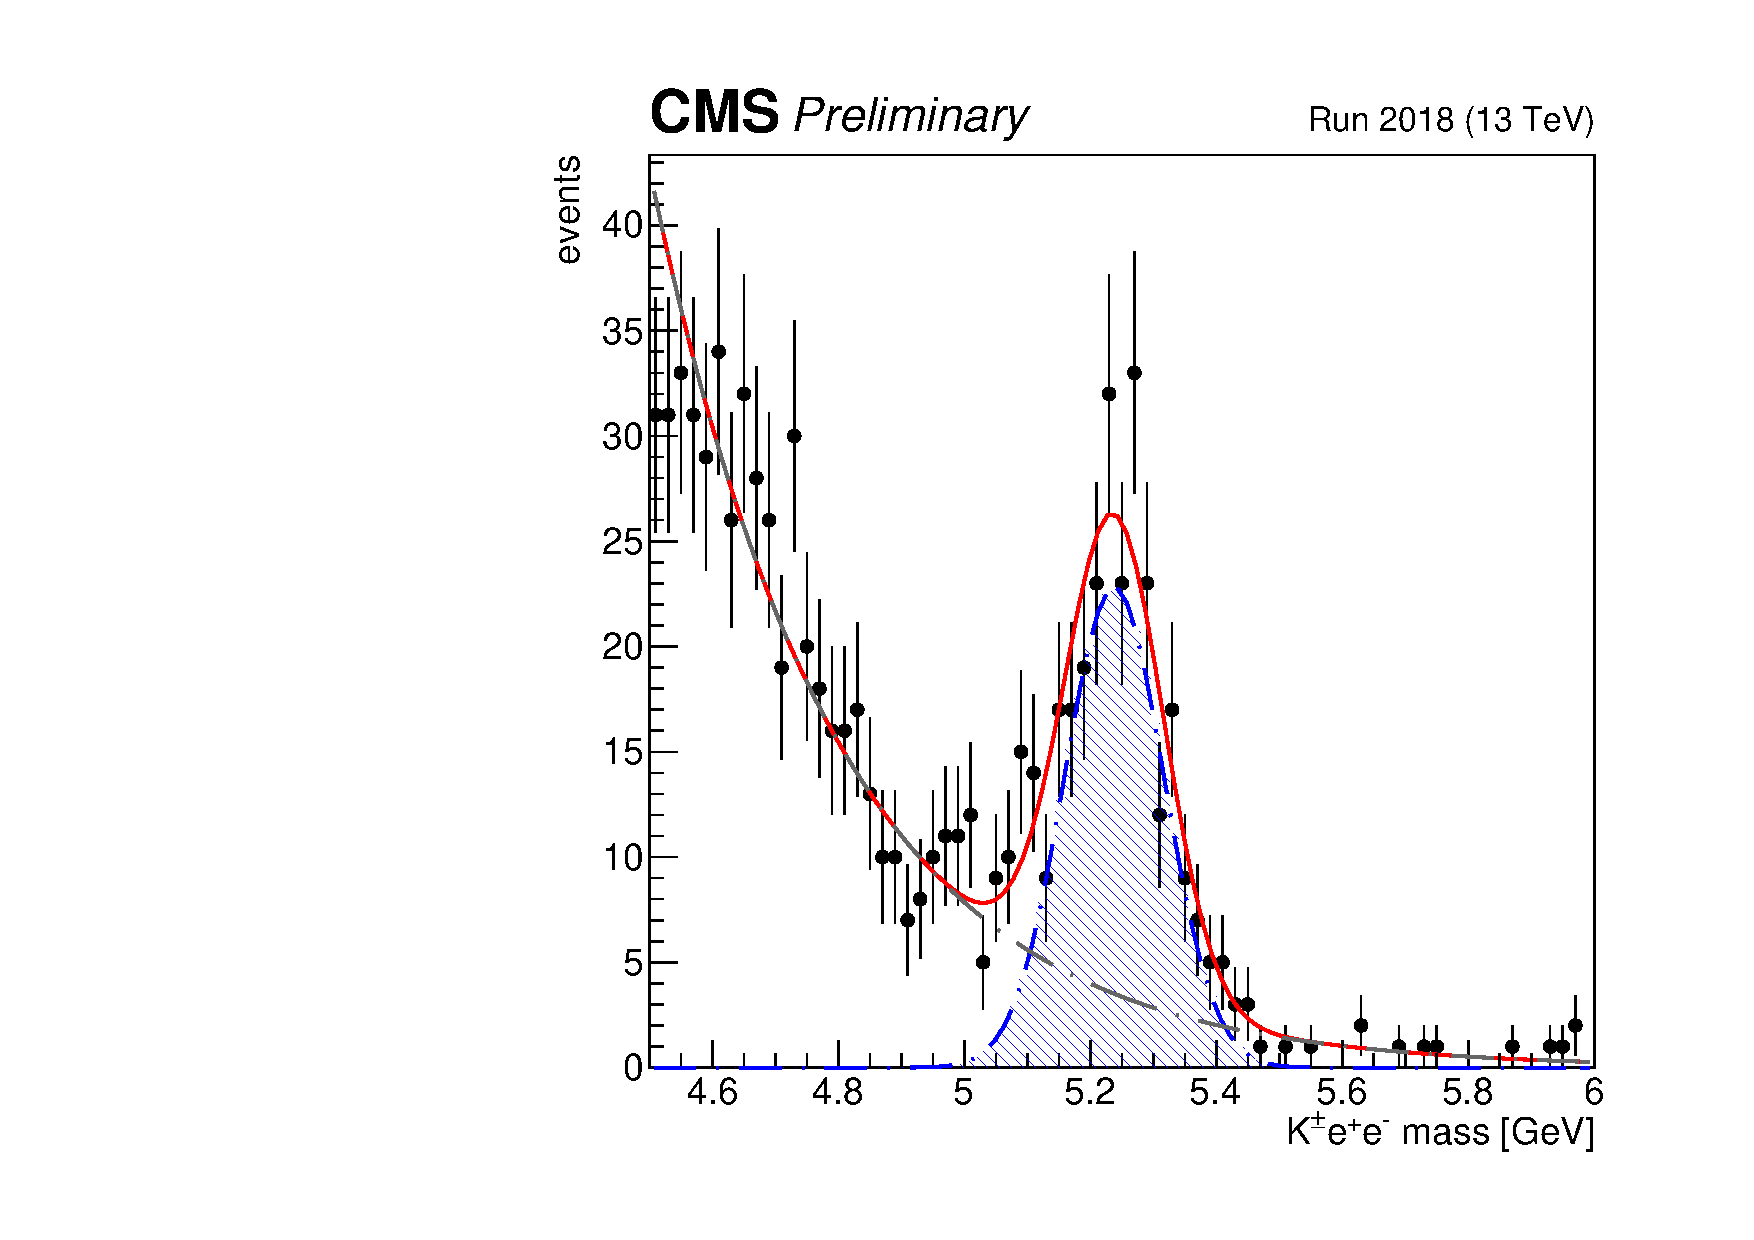
\includegraphics[width=0.45\textwidth,height=0.3\textwidth]{CMS-DP-2019-XXX_S11}
  \caption{\textbf{Left panel:} the trigger rates of the CMS HLT system as a
    function of time during an LHC fill in 2018, for the physics
    (black data points) and B parking (blue data points) streams. 
    \textbf{Right panel:} Taken from Ref.~\cite{bpark-dps}.}
  \label{fig:2} \end{figure} 

\section{Data parking}
\label{sec:3}

The DAQ system is able to handle the additional load from the B
parking stream up to a limitation determined primarily by the transfer
of the from local storage buffers at Point~5 to tape resources
available via the Tier0 centre. The trigger strategy outlined in
Sec.~\ref{sec:2} delivers a rate of ${\approx}$2~kHz when averaged
over an LHC fill, which corresponds to a throughput of
${\approx}$2\gbs. This throughput, when averaged over a timescale of
several days, can be sustained without compromising the performance of
the CMS DAQ system. 
% , such as filling to capacity the local storage buffers at P5.
The allocation of higher rates later in the LHC fills helps to
load-balance the DAQ system.

At the beginning of the LHC Run~2, CMS allocated tape resources to
accommodate the parking of data (and a copy) at an average rate of
${\approx}$500~Hz during 2016, 2017, and 2018 to support the analysis
of the scouting data stream~\cite{parking-dps}. The resources for 2017
and 2018 were reallocated to accommodate the new B parking proposal.
Assuming a single copy, these resources are sufficient to permanently
store the B parking data stream.

\section{Event reconstruction and validation}
\label{sec:4}

The B parking sample was accumulated during the period June--November
2018. The sample comprises 12~B events, recorded with high purity
triggers, and contains ${\approx}10$~B unbiased b hadron decays. The
size of the single-copy unprocessed data sample is 7.6~PB. The
reconstruction of the B parking sample occurred during the LHC long
shutdown, in the period May--December 2019. The sample is permanently
available as an analysis-level data format (MINIAOD) with a reduced
footprint. Table~\ref{tab:2} summarises the composition of the sample. 

\begin{table}[!t]
  \small%\scriptsize
  \centering
  \caption{Summary of the expected yields for important signal-side b
    hadron production (and decay) modes in the B parking data sample.
    The quoted yields are based on the same assumptions used to
    evaluate Equation~\ref{equ:2} in Sec.~\ref{sec:2}, and do not
    account for \ate. The branching fraction $\mathcal{B}$ is stated
    where appropriate, and $f_{\textrm{B}}$ is defined in the text 
    (Sec.~\ref{sec:2}). Table contents taken from
    Ref.~\cite{bpark-dps}. 
  \label{tab:2}
  } 
  %\renewcommand{\arraystretch}{1.3}
  \begin{tabular}{lr@{$\:\times\:$}lcc}
    \hline
    Mode                           & 
    \multicolumn{2}{c}{Expected yield} & 
    $f_{\textrm{B}}$                 & 
    $\mathcal{B}$                                                                                \\
    \hline
    \multicolumn{5}{c}{Generic b hadrons}                                                        \\
    $B^0_\textrm{d}$               & 4.0                      & $10^9$    & 0.4   & --          \\
    $B^\pm$                        & 4.0                      & $10^9$    & 0.4   & --          \\
    $B_\textrm{s}$                 & 1.2                      & $10^9$    & 0.1   & --          \\
    b baryons                      & 1.2                      & $10^9$    & 0.1   & --          \\
    $B_\textrm{c}$                 & 1.0                      & $10^7$    & 0.001 & --          \\
    Total                          & 1.0                      & $10^{10}$ & 1.0   & --          \\
    \hline
    \multicolumn{5}{c}{Events for \rk and \rkst analyses}                                  \\
    \btokstll                      & \multicolumn{2}{c}{2600} & 0.4       & $6.6 \times 10^{-7}$ \\
    \btokll                        & \multicolumn{2}{c}{1800} & 0.4       & $4.5 \times 10^{-7}$ \\
    \hline
  \end{tabular}
\end{table}

Approximately 7\% of the data sample, enriched in dielectron final
states from \bsll transitions, is also temporarily available in the
raw and AOD data formats, which permits further developments of
algorithms and validation studies. A "pilot" reconstruction campaign,
comprising a small fraction of the full data set, $\mathcal{O}(1\%)$,
was undertaken early in the data taking period to allow the validation
of the trigger and parking strategies. The right panel of
Fig.~\ref{fig:3} shows the invariant mass distribution obtained from
candidate \btokjpsiee decays using the standard CMS reconstruction
software. This is the first observation from CMS of \bsll transitions
in the dielectron final state, obtained from the pilot campaign, which
demonstrates the rich physics potential of the B parking sample. The
trigger purity studies, based on the reconstructed $\textrm{D}^{*+}$
candidates, were also based on the pilot campaign.

\section{Electron reconstruction}
\label{sec:5}

A crucial component of the \rk and \rkst measurements is the ability
to efficiently identify electrons down to very low transverse momenta.
The left panel of Fig.~\ref{fig:3} shows the generator-level \pt
distributions for the daughter particles from \btokll decays. The \pt
distributions are very soft, with those for the kaon and subleading
lepton peaking at ${\approx}$1~GeV. The right panel of
Fig.~\ref{fig:3} shows the efficiency to reconstruct electrons as a
function of the generator-level \pt, as obtained with the CMS default
electron reconstruction algorithm (blue square markers). The
efficiency is essentially zero for the region $0 < \pt < 2$~GeV and in
the range 0.2--0.8 for the region $2 < \pt < 10$~GeV.

\begin{figure}[!t]
  \centering
  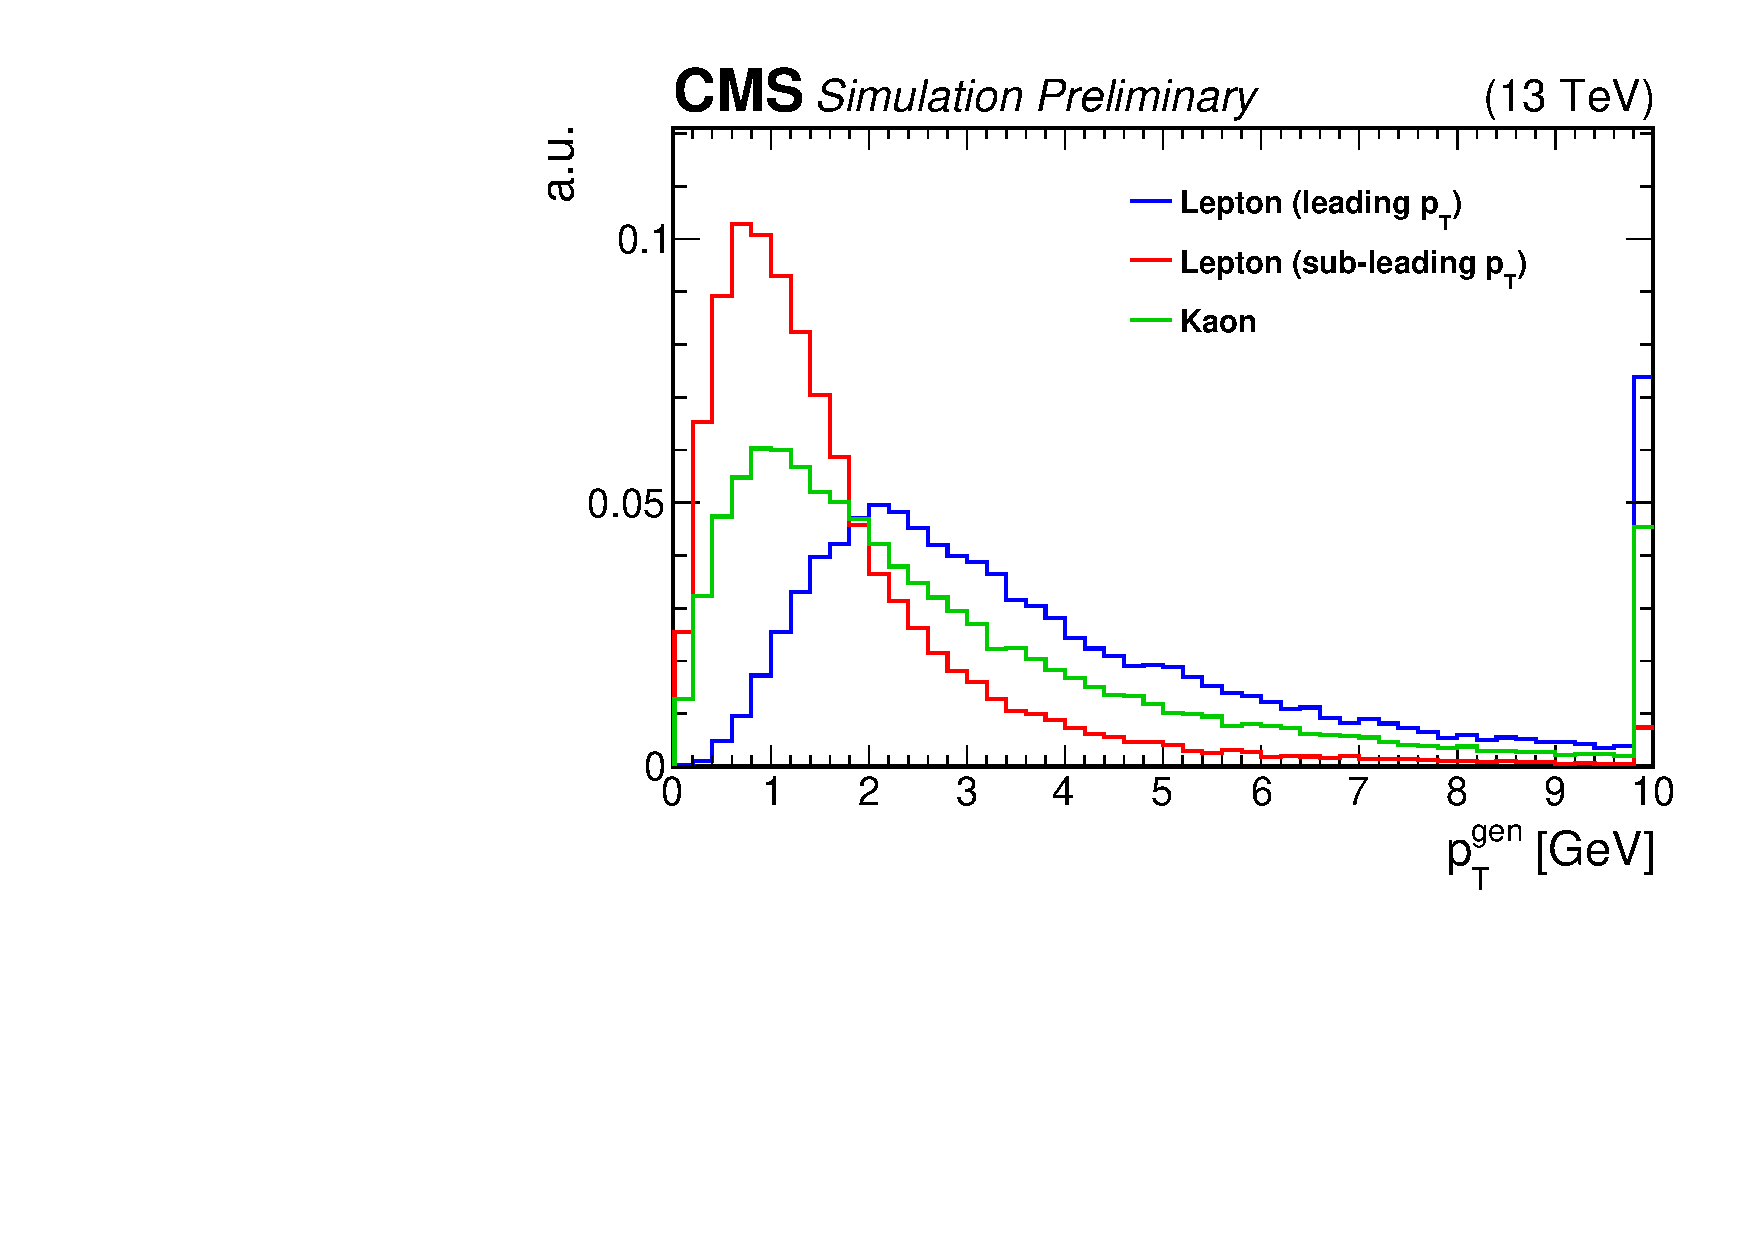
\includegraphics[width=0.45\textwidth]{CMS-DP-2019-XXX_S12}
  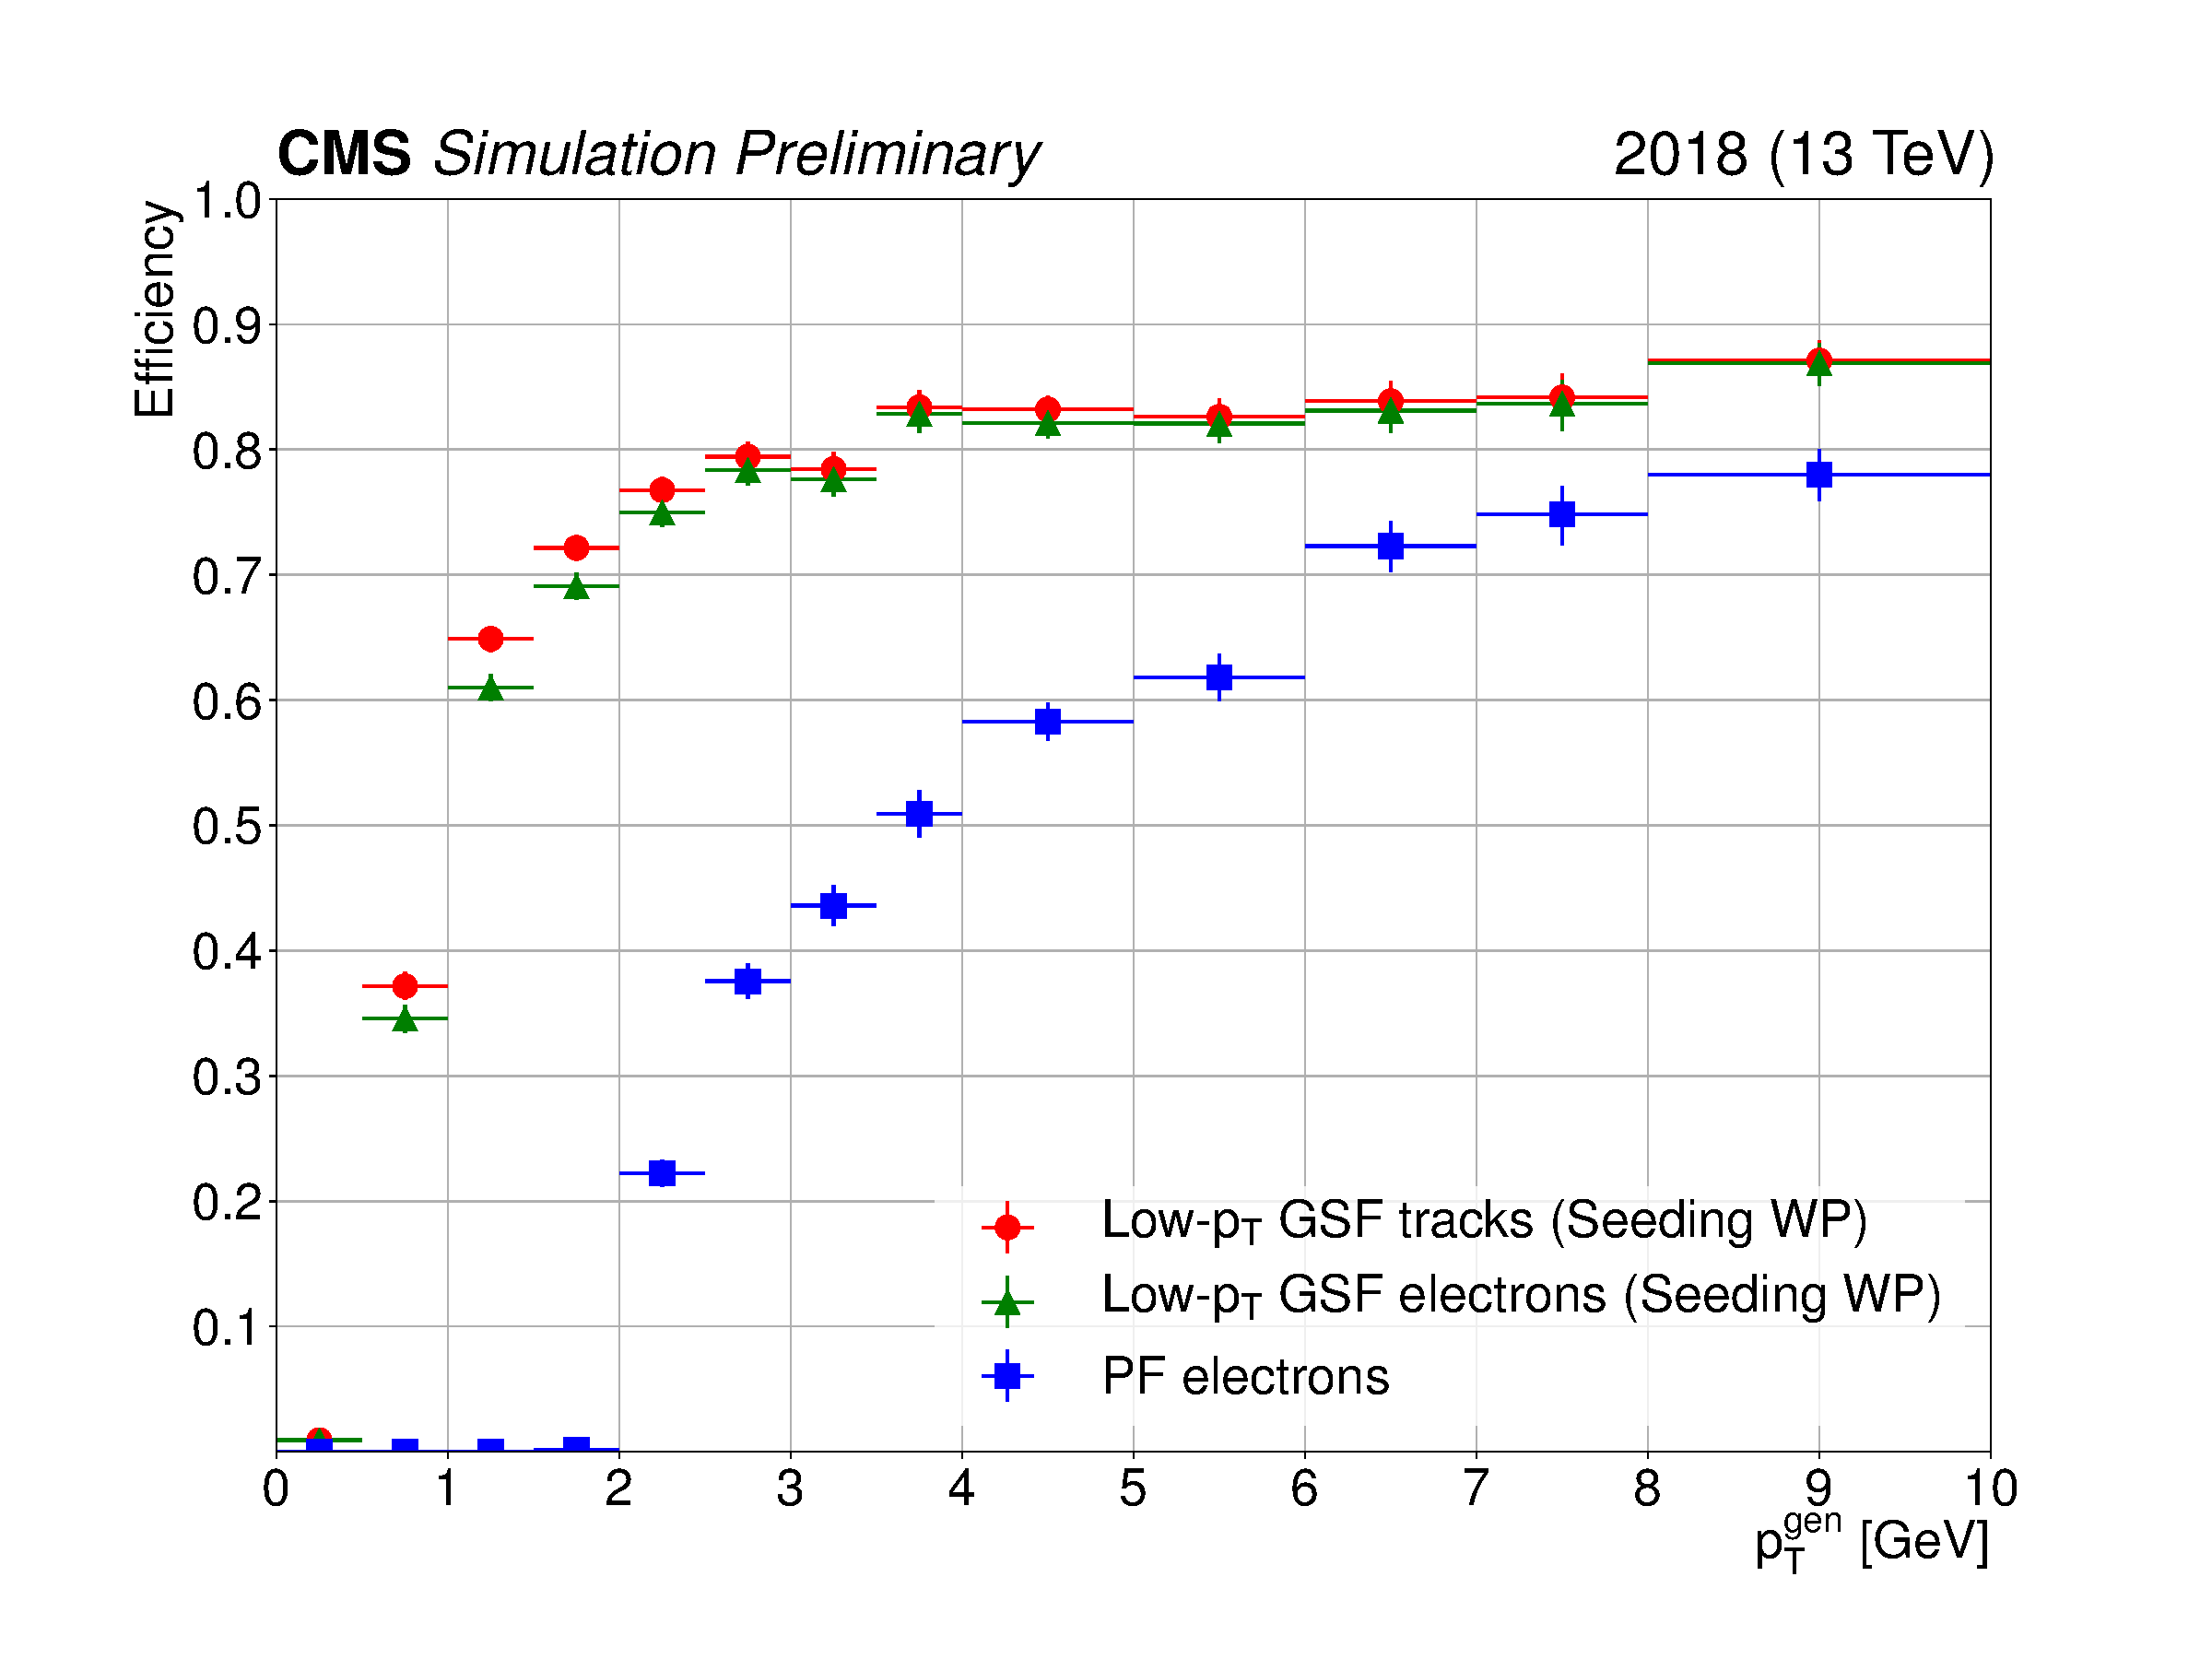
\includegraphics[width=0.45\textwidth]{CMS-DP-2019-XXX_S14}
  \caption{\textbf{Left panel:} Generator-level \pt distributions of
    the daughter particles from signal-side \btokll decays.
    \textbf{Right panel:} Reconstruction efficiency curves for standard 
    CMS electron candidates (blue squares) and for GSF tracks (red
    circles) and electron candidates (green triangles) from the new
    algorithm  as a function of the generator-level electron \pt.
    Taken from Ref.~\cite{bpark-dps}.} 
  \label{fig:3}
\end{figure}

\begin{figure}[!t]
  \centering
  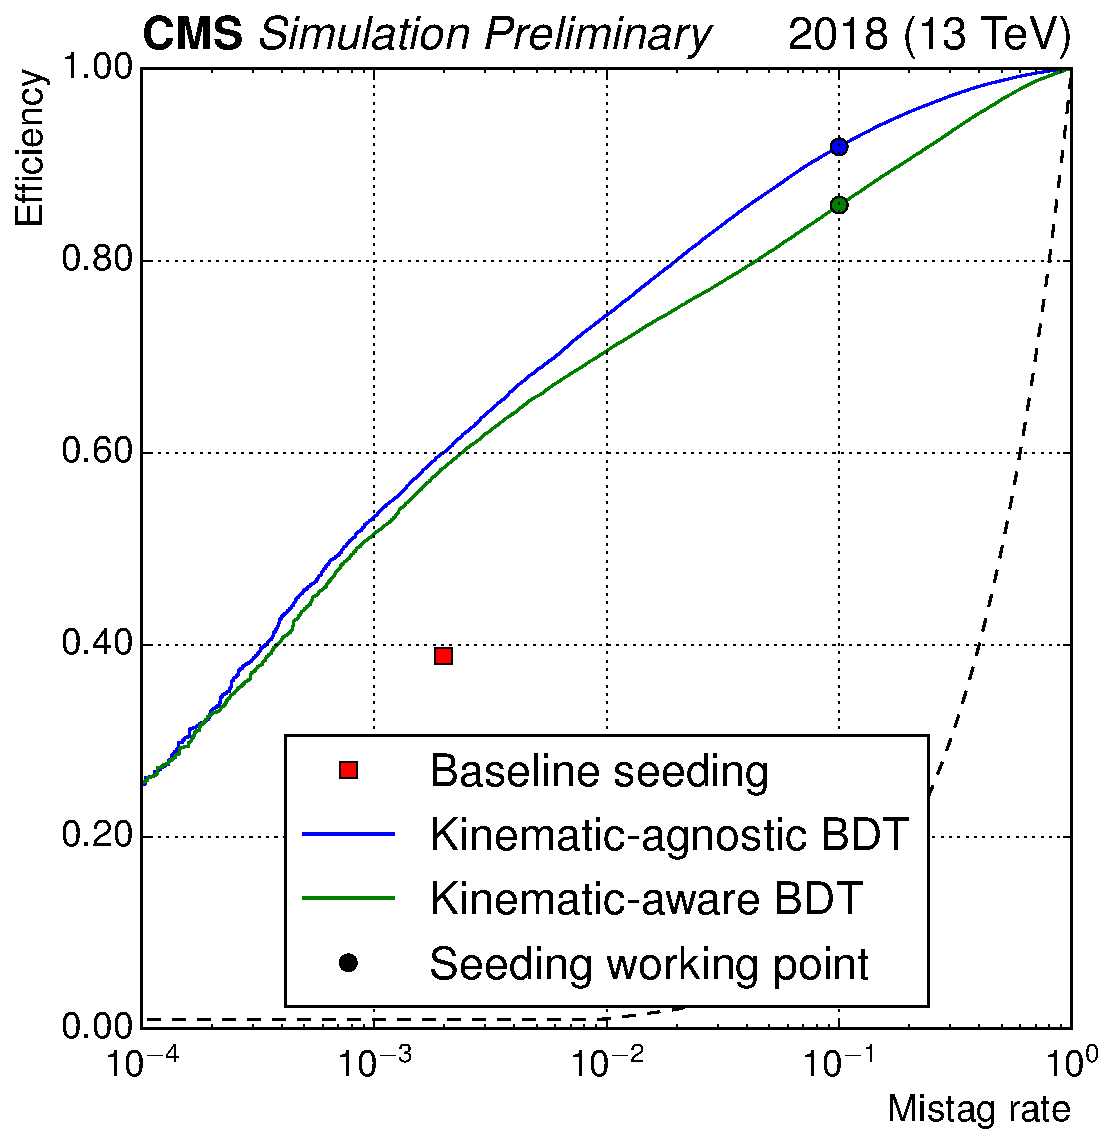
\includegraphics[width=0.45\textwidth,height=0.44\textwidth]{CMS-DP-2019-XXX_S13}
  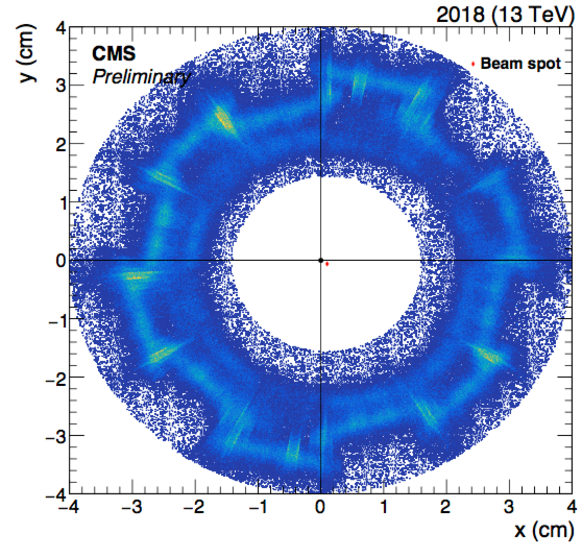
\includegraphics[width=0.45\textwidth]{CMS-DP-2019-XXX_S16_small}
  \caption{\textbf{Left panel:} ROC curves for a "kinematically
    agnostic" BDT (green curve) and a model-dependent "kinematically
    aware" BDT (blue curve), obtained from simulated \btokee events.
    Various working points, described in the text, are also indicated.
    \textbf{Right panel:} Vertex positions of photon conversion
    candidates in the transverse plane for the region $|\eta| < 1$.
    Taken from Ref.~\cite{bpark-dps}.} 
  \label{fig:4}
\end{figure}

A custom electron reconstruction algorithm, optimised for the low-\pt
regime, has been developed for the B parking data set. As for the
standard CMS electron algorithm, the determination of the
charged-particle track parameters for electron candidates, in the
presence of bremsstrahlung energy loss, relies on the use of a
Gaussian sum filter (GSF) approach~\cite{}. The "GSF tracking" stage
is computationally expensive, and therefore it is seeded by a more
computationally efficient logic that identifies potential electron
candidates. The trajectory of each GSF track is used to identify a
compatible "seed" cluster of energy in the CMS electromagnetic
calorimeter. Additional clusters of energy, consistent with the
bremsstrahlung energy loss pattern of the electron candidate, are
associated with the seed cluster as part of a "super cluster", which
can be used with the tracking information to identify genuine electron
candidates with high efficiency and purity. The right panel of
Fig.~\ref{fig:3} illustrates the increase in efficiency obtained with
the new electron reconstruction algorithm with respect to the
standard algorithm with only minimal identification quality criteria
applied.

The seeding logic implements two independent models based on boosted
decision trees (BDT). The first BDT provides signal-to-background
discrimination based on a "kinematically agnostic" approach that
exploits only tracking and calorimeter information. The second BDT
provides a (model-dependent) "kinematically aware" model that also
uses the \pt, $\eta$, and track impact parameter of an electron
candidate to discriminate signal from background. The left panel of
Fig.~\ref{fig:4} shows the ROC curves obtained for the two BDTs based
on simulated \btokee events. A loose working point is defined for each
BDT that yields a 10\% mistag rate while providing a factor
${\approx}$2 gain in efficiency over that obtained from the baseline
seeding logic of the standard CMS algorithm. These working points were
used to seed the new electron reconstruction sequence as part of the
reconstruction campaign described in Sec.~\ref{sec:4} and the
electrons are available for analysis in the MINIAOD data format.

A large, high purity sample of electrons with $0.5 < \pt < 10$~GeV can
be obtained from converted photons resulting from interactions with
the beam pipe and inner tracking structures. This sample is being used
to study and tune the identification algorithm for low-\pt electrons.
The right panel of Fig.~\ref{fig:4} shows the vertex positions of
photon conversion candidates in the transverse plane for the region
$|\eta| < 1$. The structures of the beam pipe and inner layer of the
CMS pixel barrel subdetector are clearly visible.

\section{Summary}
\label{sec:6}

The CMS experiment has recorded and reconstructed a high-purity sample
of 10 billion unbiased b hadron decays. This sample was recorded with
minimal impact on the core CMS physics programme, as the strategy
exploited the use of existing infrastructure, trigger algorithms, and
idle resources available during the latter part of LHC fills. The data
stream was parked during 2018 and processed during 2019. A new
electron reconstruction algorithm was deployed as part of the
processing campaign, which provides the potential for highly efficient
electron identification at transverse momenta as low as 0.5 GeV. This
unprecedented sample provides a unique opportunity for physics
analyses in the flavour sector and beyond.

\begin{thebibliography}{}
%% Journal Author, Journal \textbf{Volume}, page numbers (year)

\bibitem{babar} 
BaBar Collaboration, Nucl. Instrum. Meth. A \textbf{479} 1 (2002)

\bibitem{belle} 
Belle Collaboration, Nucl. Instrum. Meth. A \textbf{479} 117 (2002)

\bibitem{lhcb} 
LHCb Collaboration, JINST \textbf{3} S08005 (2008) 

\bibitem{hflav-rdrdst} 
HFLAV Collaboration, \url{https://hflav-eos.web.cern.ch/hflav-eos/semi/spring19/r_dtaunu/rdrds_spring2019.pdf} (2019) 

\bibitem{altmannshofer} 
W. Altmannshofer \textit{et al}, Phys. Rev. D \textbf{96} 055008 (2017)

\bibitem{cms-expt} 
CMS Collaboration, JINST \textbf{3} S08004 (2008)

\bibitem{bsmumu} 
CMS and LHCb Collaborations, Nature \textbf{522} 68 (2015)

\bibitem{p5prime-cms} 
CMS Collaboration, Phys. Lett. B \textbf{781} 517 (2018) 

\bibitem{cms-trigger} 
CMS Collaboration, JINST \textbf{12} P01020 (2017)

\bibitem{parking-dps} 
CMS Collaboration, CMS-DP-2012-022, \url{https://cds.cern.ch/record/1480607} (2012)

\bibitem{alphat} 
CMS Collaboration, Phys. Lett. B \textbf{767} 403 (2017)

\bibitem{bpark-dps} 
CMS Collaboration, CMS-DP-2019-043, \url{https://cds.cern.ch/record/2704495} (2019)

\end{thebibliography}

\end{document}
